
\chapter{Scope}
Die Moduldokumentation beschreibt die Architektur, die Schnittstellen
und die Hauptmerkmale des Moduls. Außerdem werden die Modul bzw. Komponententests
einschließlich der Ergebnisse beschrieben und dokumentiert.
Die MOD dient bei Bedarf auch als Programmier- oder Integrationshandbuch für das
Modul. Wenn bestimmte Risiken direkt mit der Verwendung des Moduls verknüpft sind,
so sind sie in diesem Dokument zu benennen und zu kommentieren.

\chapter{Definitionen}

\section{Abkürzungen}
DTD - Data Type Definition\\
XML - eXtensible Markup Language
JUnit - Java Unit Test
JavaDoc - Java Documentation

\section{Definitionen}
\paragraph{Maven} Ein Build-Management-Tool der Apache Software Foundation und basiert auf Java. Mit ihm kann man insbesondere Java-Programme standardisiert erstellen und verwalten.
\paragraph{Sonar} Sonar vereint die Funktionen von diverser Tools zur statischen Code-Analyse unter einem Dach und bietet eine komfortable Web-Oberfläche zur Auswertung der gesammelten Statistiken an.%Wichtige Begriffe und Worte

\section{Terminologien}
Struktur von XML Dokumenten: DTD

\chapter{Analyse}

\section{Voruntersuchungen}

Für den Controller mussten keine Prototypen, anfänglichen Versuche, Tests oder Abschätzungen gemacht werden.\\
Der Controller dient als Schnittstelle bzw. Bindeglied zwischen dem Model und den Views. \\
Ein früher Prototyp des Models konnte somit bereits im Vorfeld ohne einen Prototyp des Controllers realisiert werden.

\section{Systemanalyse}

\subsection{Rahmenbedingungen}
Der Controller stellt das Bindeglied zwischen Model und View da. Er dient zum Einen zum Initialisieren des Programms, zum Anderen im selbigen Zug
zum Instantiieren des Models und der Views.\\
Zusätzlich nimmt der Controller bestimmte Verwaltungsaufgaben war. Dazu zählt in etwa die Profilverwaltung, das Fehlerverwaltungssystem und die Sprachverwaltung.\\
Als Bindeglied zwischen Model und View muss er zusätzlich als Stream-Manager agieren und Observeranfragen von der View an das Model durchreichen.\\
Da er sich um den Aufbau des Programms kümmert muss er sich analog auch um den korrekten Abbau des Programms kümmern.

\subsection{Problemstellung}
Die Problemstellung bestand daher aus mehreren Teilen. Es waren Fragen zu klären wie:

\begin{enumerate}
  \item Wie werden Profile gespeichert?
  \item Wie werden Profile geladen?
  \item Wie erfahren Teile des Programms, dass ein neues Profil geladen wurde?
  \item Wie werden kürzlich benutzte Profile gespeichert und geladen?
  \item Wie werden kürzlich benutzte Profile verwaltet?
  \item Wie erfahren Teile des Programms, dass die Sprache geändert wurde?
  \item Wie wird eine Kommunikation zwischen View und Model ermöglicht?
  \item Wie können mehrere Views ermöglicht werden?
  \item Wie erfährt die View Updates über das Model?
  \item Wie werden Fehler berichtet?
  \item Wie werden Fehler kategorisiert?
  \item An wen wird ein berichteter Fehler weitergereicht?
  \item Wie kann das Programm über Startparameter gestartet werden?
  \item Was soll alles über die Startparameter konfigurierbar sein?
  \item Wie ist der Syntax für die Startparameter?
  \item Wie wird das Programm korrekt beendet?
\end{enumerate}

\subsection{Gliederung der Komponente}
Um die Fragen zu lösen musste eine passende Architektur für den Controller ausgearbeitet werden. Bereits in der
SAS wurde der Controller spezifiziert. Es fehlten jedoch wichtige Teile wie die Fehlerberichterstattung.
Ebenfalls mussten manche Interfaces angepasst werden, um eine Lösung zu ermöglichen.

Die Aufgaben des Controllers können somit in folgende Hauptpunkte unterteilt werden:

\begin{enumerate}
  \item Starten des Programms mit Startparameter und Initialisierung des Models und der View
  \item Speichern/Laden von Profilen
  \item Verwaltung von kürzlich benutzten Profilen
  \item Ermöglichen der Kommunikation zwischen Model und View
  \item Weitergabe von Sprachänderungen
  \item Verwaltung und Weitergabe von berichteten Fehlern
  \item Korrektes Beenden des Programms
\end{enumerate}

\subsection{Abhängigkeiten zu anderen Modulen}
Als "`Initiator"' des Programms steht der Controller mehr oder minder in Abhängigkeit zu allen anderen Modulen.
Als Schnittstelle zwischen Model und View ergibt sich implizit eine Abhängigkeit zum Modul "`Gui-Logik"' und zum Modul "`Model"'.
Da das Modul "`CLI/Logger"' eine weitere Realisierung des Abstrakten Begriffs "`View"' darstellt besteht auch hierzu eine Abhängigkeit.\\
Durch Verwaltung der Sprache besteht eine Verknüpfung zum Modul "`Language"'. Das Modul "`Package"', "`Installer"' oder "`Gui-Design"' stehen nur sehr
Indirekt in Verbindung mit dem Controller und können daher vernachlässigt werden.

\chapter{Design}

\section{Folgerungen}
Wie sich deutlich in der Analyse erkennen lässt, ist der Controller der "`Kleber"', der das Programm zusammen hält und über den sämtliche Kommunikation zwischen den Modulen
"`Model"',"'Gui-Logik"' und "`CLI-Controller"' zunächst abläuft.\\
Um sämtliche Verteilung von Daten, Änderungen der Sprache oder Profilen und Fehlerberichterstattungen zu ermöglichen wurde daher exzessiv das Observer Designpattern verwendet.
Da es jeweils im Programm nur einen Controller geben darf wird dieser als Singleton in der Architektur realisiert.\\
Die Speicherung von Daten erfolgt ausschließlich im XML Format.\\
Der Einstiegspunkt des Programms wird definitiv Teil des Controller werden, welche diesen Starten und anschließen die Kontrolle über das Programm an ihn übergibt.

\section{Lösungen für die Problemstellungen}

  \paragraph{Wie werden Profile gespeichert?}
  Profile sollen später vom Benutzer zu öffnen sein, um sie betrachten und editieren zu können.
  Die Profile müssen also in einem "`human-radable"' Format gesichert werden. Hierfür wird XML verwendet
  und bei der Abspeicherung zusätzlich auf korrektes Einrücken geachtet, so dass die Daten dem Benutzer noch strukturierter dargestellt werden.\\
  Das folgende Listing zeigt die DTD der abzuspeichernden XML Datei. \#PCDATA ist ein Platzhalter für jegliche Art von Daten. \#IP ist ein Platzhalter für eine IP-Adresse
  und \#NUMBER ein Platzhalter für eine Nummer im Dezimalsystem.\\

  \lstinputlisting[frame=single,label=dtd,caption=Profile DTD,language=XML,numbers=none]{listing/dtd.txt}
  Das erzeugte Profil muss anschließend unter dem vom Benutzer gewählten Pfad gesichert werden.
  Dabei stehen die verwendeten Abkürzungen im Bereich Sender/Receiver später für folgende Attribute:

  \begin{table}[H]
    \label{tap:types}
    \caption{Atrribute und Beschreibungen}
    \center
    \begin{tabular}{|c|p{8cm}|}
    \hline
    \textbf{Attribut} & \textbf{Bechreibung}\\
    \hline
    active & Gibt an, ob ein Sender/Empfänger bei der Speicherung aktiv war\\
    \hline
    psize & Paketgröße in Bytes\\
    \hline
    port & Portnummer\\
    \hline
    pps & Pakete pro Sekunde (Senderate)\\
    \hline
    ninf & Network Interface - IP Adresse des zu verwendenten Netzwerkinterfaces\\
    \hline
   	abeh & Anazlyzing Behaviour - Analyseverhalten der Messwerte\\
    \hline
   	ptype & Package Type - SPAM oder Hirschmann Pakete\\
    \hline
    ttl & Time to life\\
    \hline
    payload & Nutzdaten\\
    \hline
    group &  Multicast Gruppen IP\\
    \hline
    \end{tabular}
  \end{table}

  \paragraph{Wie werden Profile geladen?}
  Das Profilladen erfolgt analog zum Speichern mittels der Profildatei in dem im DTD angegebenen XML Format.
  \paragraph{Wie erfahren Teile des Programms, dass ein neues Profil geladen wurde?}
  Das Controller muss andere Teile des Programms, z.B. die GUI oder den Logger über einen Profilwechsel informieren. Hierzu wird das Observer-Pattern benutzt.
  Interessenten registrieren sich als "`Listener"' bei dem Controller, welcher bei einem Profilwechsel eine spezielle Funktion bei Ihnen aufruft.
  \paragraph{Wie werden kürzlich benutzte Profile gespeichert und geladen?}
  Kürzlich benutzte Profile müssen nicht in einem "`human-readable"' Format gespeichert werden. Die Implementierung ist somit egal.
  Es müssen immer Paare aus Profilname und Profilpfad gesichert werden. Diese Liste muss zum Programmstart eingelesen werden und bei jeder Änderung sicherheitshalber gesichert werden.
  Das sofortige Sichern beseitigt den Verlust von allen Änderungen beim Programmabsturz.
  \paragraph{Wie werden kürzlich benutzte Profile verwaltet?}
  Die Liste muss strukturiert verwaltet werden. Wird ein neues Profil gespeichert, so wird es ganz oben in der Liste eingefügt.
  Wird ein existierendes Profil geladen oder erneut gesichert, so wandert es in der Liste ganz nach oben. Überschreibt der Benutzer ein Profil mit
  einem Profil mit anderem Namen, so muss der alte Eintrag aus der Liste entfernt werden. Um die Übersichtlichkeit zu erhalten werden maximal 10 Profile in die Liste aufgenommen.
  Um entfernte Profile zu erkennen und die Liste von diesen zu bereinigen wird nach jedem Laden der Liste(beim Programmstart) überprüft, ob die einzelnen referenzierten Profildateien noch existieren.\\
  Wenn nicht, wird das jeweilige Profil aus der Liste entfernt.
  \paragraph{Wie erfahren Teile des Programms, dass die Sprache geändert wurde?}
  Auch hierbei wird analog zur Profiländerung das Observer-Designattern verwendet.
  \paragraph{Wie wird eine Kommunikation zwischen View und Model ermöglicht?}
  Will eine View über Updates des Models erfahren, so kann sie sich indirekt über den Controller bei dem Model als "`Listener"' registrieren.\\
  Der Controller leitet die Registrierung/Deregistrierung jeweils nur weiter. Die folgende Kommunikation erfolgt ohne Einbezug des Controllers.
  \paragraph{Wie können mehrere Views ermöglicht werden?}
  Mehrere Views können über das Observer-Designpattern ermöglicht werden. Der Controller instantiiert die Views jeweils, welche sich darauf hin über den Controller beim Model als "`Listener"' eintragen.
  \paragraph{Wie erfährt die View Updates über das Model?}
  Über die indirekte Registrierung beim Model als "`Listener"' über den Controller. Die Verwendung des Observer-Patterns findet hierbei im Model statt. Der Controller
  leitet die Anfragen nur weiter.
  \paragraph{Wie werden Fehler berichtet?}
  Um Fehler zu berichten wird analog zu Sprachänderungen und Profiländerungen das Observer-Designpattern verwendet. Über den Controller werden ErrorEvents gemeldet.
  Der Controller verteilt die ErrorEvents anschließend an "`Listener"', die an den Kategorieren der ErrorEvents interessiert sind.
  \paragraph{Wie werden Fehler kategorisiert?}
  Eine Kategorisierung erfolgt anhand der Kritikalität. Dafür stehen 6 Stufen bereit:
  \begin{table}[H]
    \label{tap:cat}
    \caption{Fehlerkategorisierung}
    \center
    \begin{tabular}{|c|c|}
    \hline
    \textbf{Abkürzung} & \textbf{Stufe}\\
    \hline
    DEBUG & 0\\
    \hline
    WARNING & 1\\
    \hline
    SEVERE & 2\\
    \hline
    ERROR & 3\\
    \hline
    CRITICAL & 4\\
    \hline
   	FATAL & 5\\
    \hline
    \end{tabular}
  \end{table}

  \paragraph{An wen wird ein berichteter Fehler weitergereicht?}
  Bei dem Controller können sich "`Listener"' registrieren, welche über ErrorEvents informiert werden können.
  Ein "`Listener"' kann sich unter einer bestimmten Kategorie eintragen. Er wird anschließend nur über ErrorEvents informiert, die auf selbem Level oder darüber liegen.
  \paragraph{Wie kann das Programm über Startparameter gestartet werden?}
  Das Programm wird über die Kommandozeile gestartet, wobei dabei Argumente bzw. Startparameter angegeben werden. Eine weitere Konfiguration
  des Programms über die Kommandozeile während der Programmausführung ist nicht möglich.
  \paragraph{Was soll alles über die Startparameter konfigurierbar sein?}
  Das Programm muss über Startparameter gestartet werden können. Es muss möglich sein die GUI auszuschalten, den Logger einzuschalten, Profile zu laden und
  Streams der geladenen Profile automatisch zu starten.
  \paragraph{Wie ist der Syntax für die Startparameter?}
  Tabelle 4.1  zeigt die Übersicht der Startparameter.
  \begin{table}[H]
    \label{paramter}
    \caption{Startparameter des Programms}
    \center
    \begin{tabular}{|p{5cm}|p{10cm}|}
    \hline
    \textbf{Befehl} & \textbf{Beschreibung}\\
    \hline
    -nogui & Startet das Tool ohne GUI\\
    \hline
    -cli & Startet den Logger mit\\
    \hline
    -profile <PROFILNAME> & Lädt ein oder mehrere Profile anhand des
    Profilnamens (getrennt durch Leerzeichen)\\
    \hline
    -path <PATH> & Lädt ein oder mehrere Profile anhand eines Pfades (getrennt durch
    Leerzeichen)\\
    \hline
    -startall & Startet alle Sender/Empfänger der geladenen Konfigurationen\\
    \hline
    -startnone & Startet keine der Sender/Empfänger der geladenen Konfigurationen\\
    \hline
    -restore & Startet alle Sender/Empfänger in dem Status (aktiv/inaktiv), wie im
    Profil gespeichert (default)\\
    \hline
    \end{tabular}
  \end{table}
  Die Parameter können ohne definierte Reihenfolge verwendet werden. Es ist nicht möglich das "`Startverhalten"' der Streams mehrfach zu definieren.
  \paragraph{Wie wird das Programm korrekt beendet?}
  Damit das Programm korrekt beendet werden kann muss der Controller eine Funktion bereitstellen, die das Programm strukturiert beendet.
  Es müssen alle GUI's beendet werden, der Logger beendet werden und das Model beendet werden. Dies stellt einen korrekten Programmfluss beim Beenden sicher.\\
  So werden etwa Logdateien richtig geschrieben und Fehler beim Beenden vermieden.

\section{Systemarchitektur, Interfaces und Schnittstellen}

  Die Architektur des Controller ist in Abbildung \ref{img:sysarch} aufgeführt. Man sieht deutlich die Abhängigkeit zwischen Controller und Model im unteren Bereich(SenderPool, ReceiverPool)
  und die Zusammenarbeit zwischen Model und Gui/CLI im oberen Bereich(Zugriff der AbstractView auf verschiedene Interfaces des Controllers).
  \begin{figure}[H]
      \centering
      \fbox{
        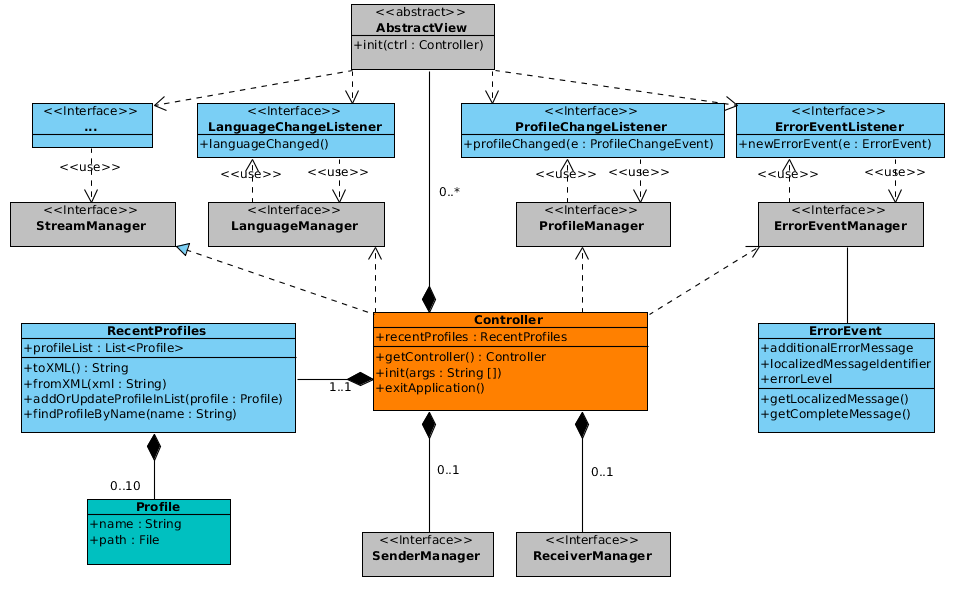
\includegraphics[width=15cm]{images/Controller.png}
      }
      \caption{Arrchitektur des Controllers}
      \label{img:sysarch}
  \end{figure}
  Die Interfaces, die der Controller implementiert, sind in Abbildung \ref{img:inter} verfeinert und näher spezifiziert.
  \begin{figure}[H]
      \centering
      \fbox{
        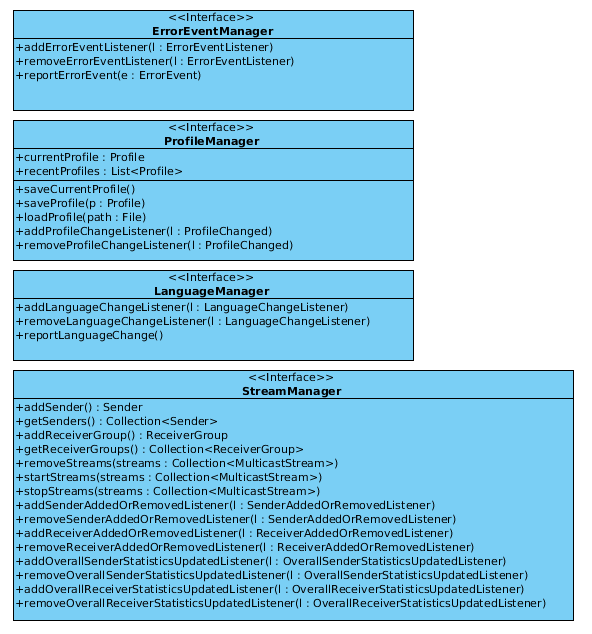
\includegraphics[width=12cm]{images/Interfaces.png}
      }
      \caption{Interfaces, die der Controller implementiert}
      \label{img:inter}
  \end{figure}
  Wie zu sehen ist, ist der Controller als Singleton designt. Es wird innerhalb des Programms immer nur einen Controller geben. Diese Designentscheidung ermöglicht es zusätzlich aus jedem Punkt des Programms auf den Controller zuzugreifen.
 \\Es wurden bereits alle Interfaces auf Funktionsebene definiert. Der Controller muss während der Implementierung nur noch diese Funktionen realisieren.
 Die Abstraktion über Interfaces ermöglicht eine geringere Kopplung der Module. Der Controller wird dadruch besser austauschbar und erweiterbar.

\chapter{Implementierung}
In diesem Abschnitt soll kurz auf die Implementierung eingegangen werden.
Details zur Implementierung sind in der Java Dokumentation JavaDoc hinterlegt.

\section{Vorgehen}
Das Vorgehen bestand daraus, zunächst die Grundfunktionalität sicher zu stellen. Dies beinhaltete das Einbinden und Ansprechen des Models und der Views.
Im weiteren Verlauf der Implementierung wurde die Profilspeicherung, Profilverwaltung und die Sprachverwaltung eingebaut.\\
Zuletzt wurde die Startbarkeit über Startparameter und die Fehlerverwaltung hinzugefügt.\\
Im Anschluss daran wurden die jeweiligen Komponenten/Modultests erstellt. Nach dem Debugging, sowie dem Testen war die Implementierungsphase abgeschlossen.\\
Das Programm Maven bzw. Sonar übernahm die Aufgabe der statischen Codeanalyse. Mit der Ausgabe wurde der Programmcode optimiert und die Coding-Standards sichergestellt.

\section{Teilbereiche des Moduls}
Die Implementierung in einer groben Strukturierung soll anhand der in der Analysephase gefundenen Hauptaufgaben aufgeführt werden.
Die Beschreibungen sind nicht vollständig sondern eher abstrakt gehalten. Details sind im Programmcode hinterlegt.\\

\paragraph{Starten des Programms mit Startparameter und Initialisierung des Models und der View}
Der Controller wird über die init() Methode initialisiert. Dazu holt sich die Main-Funktion zunächst das Controller-Singleton Objekt und initialisiert es anschließend, indem sie
der init() Methode die Programmparameter übergibt.\\
Die init() Methode initialisiert zunächst das Model, liest die Liste kürzlich verwendeter Profile ein und überprüft anschließend die übergebenen Parameter. Ist "`-nogui"' enthalten, wird das starten der GUI deaktiviert. Ist "`-cli"' enthalten, wird die CLI aktiviert.\\
Über "`-path"' bzw. "`-name"' können Profile geladen werden. Bei "`-path"' werden anschließende Argumente bis zum nächsten mit "`-"' Beginnenden Argument in eine Liste von zu ladender Profile gespeichert. Bei "`-name"' wird versucht die danach folgenden Namen
in der Liste kürzlich verwendeter Profile zu finden. Existiert solch ein Profil, wird es ebenfalls zur Liste zu ladender Profile hinzugefügt. Über "`-startall"', "`-startnone"' oder "`restore"' wird festgelegt, ob Sender und Receiver nach dem Anlegen direkt gestartet werden sollen.\\
Nach der Überprüfung der Parameter werden die ausgewählten Views gestartet und initialisiert. Darauf hin werden alle zu ladenden Profile in der Liste geladen. Unter Angabe des ausgewählten Startmode werden die Streams auch gleich gestartet, falls erwünscht.
\paragraph{Speichern/Laden von Profilen}
Zum Speichern und Laden von Profilen wird die Xerces Bibliothek verwendet. Diese bietet zum einen die Funktionalität, ein Document Objekt zu serialisieren und die Funktionalität, eine XML Datei zu parsen um ein Document Objekt zu erstellen.\\
Damit ein Profil abgespeichert werden kann, muss ein Profile Objekt übergeben werden, welches Namen des Profiles und Pfad der späteren Datei enthält. Zum Aufbau der XML Struktur wird zunächst ein DOM Dokument erstellt. Anschließend wird darin die hierarchische Datenstruktur aufgebaut.
Um die Konfiguration der Sender zu speichern wird die Liste aller Sender von dem Model geholt. Von jedem Sender kann direkt die Konfiguration in Form einer Hashmap abgefragt werden. Pro Sender wird jeweils das Key-Hash Paar abgespeichert. Anschließend wird der aktuelle Zustand des Senders abgefragt.
Dieser wird unter "`active"' als "`true"' oder "`false"' hinterlegt. Analog werden alle aktuellen Receiver gespeichert. Als letzter Schritt muss das Document Objekt nur noch mittels der Xerces Bibliothek in eine Datei im XML Format serialisiert werden.\\\newline
Das Laden eines Profils erfolgt in umgekehrter Weise. Mittels der Xerces Bibliothek wird direkt die XML Datei geladen und automatisch geparsed. Treten Fehler auf, so werden diese Fehler berichtet. Andernfalls wird zunächst der Profilname gelesen und anschließend zunächst alle Sender und dann alle Receiver geladen und gestartet, je nach Angabe des Startmode.
Zum Laden der Sender und Receiver wird jeweils eine Hashmap pro Sender/Receiver erstellt, die alle Key-Value Paare der jeweiligen Sektion in der XML Datei enthält. Diese Struktur wird an das Model übergeben, welches Sender/Receiver anlegt.\\
Jeweils nach dem Laden/Speichern eines Profils wird überprüft, ob der Vorgang erfolgreich war. Ist dies der Fall, so wird das Profil in der Liste kürzlich benutzer Profile aktualisiert.
\paragraph{Verwaltung von kürzlich benutzten Profilen}
Die Verwaltung der kürzlich benutzten Profile findet in einer eigenen Klasse statt. Der Controller legt dafür im Konstrukteur direkt ein Objekt an. Um die Liste aus der Datei zu füllen wird im Controller die
entsprechende Datei geöffnet und als String eingelesen. Dieser String wird an das RecentProfiles Objekt über die Funktion fromString() übergeben. Ähnlich erfolgt das Speichern der Liste.
Im Controller wird die entsprechende Datei geöffnet und danach die Daten als String geschrieben. Die Daten erhält der Controller über die toXML() Methode des RecentProfiles Objekt.\\
In dem Objekt selbst erfolgt die Realisierung der fromXML() bzw. toXML Methode über das XStream framework, welches eine direkte Serialisierung von Objekten, hier einer Liste, ermöglicht. Auf Details soll hier nicht näher eingegangen werden.\\
Die Verwaltung der internen Liste ist recht einfach. Ein Profil wird zu der Liste hinzugefügt bzw. geupdated indem die addOrUpdateProfileInList() Methode mit dem entsprechenden Profil aufgerufen wird.\\
Hier wird überprüft ob bereits ein Profil mit selbem Pfad existiert. In diesem Fall wird der Eintrag gelöscht. Anschließend wird das Profil an oberster Stelle in die Liste eingefügt. Sind nun mehr als 10
Elemente in der Liste, so werden die letzten Elemente entfernt. Zusätzlich existiert in dem RecentProfiles Objekt die Methode findProfileByName(), welche das Auffinden eines Profils anhand des Namens ermöglicht. Dies wird beispielsweiße in der init() Methode des Controllers benutzt.

\paragraph{Ermöglichen der Kommunikation zwischen Model und View}
Um die Kommunikation zwischen Model und View zu ermöglichen implementiert der Controller das Interface StreamManager. Fast alle Funktionsaufrufe leiten lediglich den Aufruf an das Model weiter, weshalb JUnit Tests hierfür Fehl am Platz sind.\\
Lediglich die Funktion removeStreams() stellt fest, von welchen Typ die übergebene Streams sind und ruf auf dem Model die passenden Funktionen auf.
\paragraph{Weitergabe von Sprachänderungen}
Die Implementierung für die Weitergabe von Sprachänderungen ist eher trivial. Hat ein Modul die Sprache geändert, so ruft es auf dem Controller die Methode languageChanged() auf.
Diese informiert jeden registrierten Listener per Aufruf der Funktion languageChanged() über die Sprachänderung. Da die Sprachänderung fest in Java integriert ist, muss der Controller die Änderung nicht selbst vornehmen. Die Nachricht dient
nur beispielsweiße der Gui, um sich neu zu zeichnen. Fehlermeldungen werden automatisch neu übersetzt.
\paragraph{Verwaltung und Weitergabe von berichteten Fehlern}
Für Fehler wurde die Klasse ErrorEvent eingeführt. Sie speichert einen Identifier für einen Fehler, mit dessen die übersetzte Nachricht erhalten werden kann, zusammen mit einer zusätzlichen Nachricht und einem Error Level.\\
Registriert sich ein Listener als ErrorEventListener, so muss er ein Error Level angeben, über welches er informiert werden will. Er erhält im Anschluss nur Fehlermeldungen, die ein gleiches oder höheres Error Level, wie er selbst, haben.\\
Um dies zu realisieren wird zu jedem Listener in einer Hashmap das ErrorLevel gespeichert. Wird bei dem Controller über der Funktion reportErrorEvent() ein Fehler berichtet, so wird dieses nur an diejenigen Listener verteilt, die einen passenden Eintrag in der Hashmap haben.\\
Erhält ein Listener ein ErrorEvent. so kann er darauf die Methode getCompleteMessage() aufrufen, um die übersetzte Nachricht + zusätzlicher Nachricht auf einmal zu erhalten.
\paragraph{Korrektes Beenden des Programms}
Beim Beenden des Programms muss darauf geachtet werden, dass zunächst das Model "`heruntergefahren"' wird(alle Streams geschlossen werden) und anschließend die Views korrekt beendet werden.
Hierzu wird zunächst auf dem Model, dem Sender- und ReceiverPool, die Methode killAll() aufgerufen. Diese schließt alle Streams. Anschließend wird sicherheitshalber die Liste kürzlich verwendeter Profile gespeichert.\\
Die Views können anschließend über den Aufruf der kill() Methode beendet werden. Dies speichert beispielsweise das Logfile im Logger. Das Programm kann nun beendet werden. Die Funktion, die diesen Funktionsumfang implementiert ist die Funktion exitApplication() im Controller.

\section{Dokumentation}
Der Programmcode wurde ausführlich in JavaDoc dokumentiert. Bei der Implementierung von Funktionen eines Interfaces befindet sich die Funktionsbeschreibung jeweils in dem zugehörigen Interface.\\


\chapter{Komponententest}

\section{Testvorgehen}

Die korrekte Funktionalität des Controller wird hauptsächlich über Junit-Tests, sowie System-Tests realisiert.
Die zugehörigen Testsuiten finden sich in dem STP, die zugehörigen Ergebnisse in dem STR. Die Systemtests bzw. deren Ergebnisse werden
hier aufgrund von Redundanz nicht erneut hinterlegt.\\
Die betreffenden Testsuiten lauten:
\begin{itemize}
  \item /TS30/ - Laden und Speichern der Konfiguration
  \item /TS40/ - Laden einer Konfiguration und Starten von Streams über CLI
\end{itemize}
Die beiden Testsuiten testen zum einen das Laden und Speichern von Profilen, sowie das Starten des Programms mit Startparametern.\\
Da alle anderen Testsuiten jeweils Funktionen nutzen, die entweder direkt oder indirekt von dem Controller abhängen,
testen quasi alle Testsuiten einen Teil des Controllers.\\
\newline
Mit JUnit Tests wird die Verwaltung kürzlich verwendeter Profile, Profile an sich, Sprachverwaltung , ErrorEvents und die Fehlerverwaltung getestet.\\
Andere Tests sind aufgrund der Abhängigkeit zu anderen Modulen nicht sinnvoll und wurden daher in die Systemtests ausgelagert. Viele Tests wären nicht deterministisch und daher nicht für automatisierte Tests geeignet.\\
\newline
Die JUnit Tests wurden konzipiert, möglichst jede Funktionalität des zu testenden Teils abzudecken. Die Tests werden automatisiert von Maven ausgeführt
und ermöglichen somit eine stetige Überprüfung der korrekten Funktionalität der entsprechenden Komponente.
Die Dokumentation wird somit auch in Maven vorgenommen. Hier werden die Testergebnisse nach vollendeter Implementierung dargestellt.
Alle Tests befinden sich in "`src/test/java/com/spam/mctool/controller"'. Nähere Erläuterungen zu den Tests sind dort hinterlegt.

\section{Komponententestplan und Komponententestreport}

\begin{table}[h]
\caption{Komponententestplan}
\label{tab:ktp}
\begin{center}
\begin{tabular}{|p{2cm}|p{5cm}|p{7cm}|}
\hline
\textbf{Test Nr.} & \textbf{Beschreibung} & \textbf{Test Klasse}\\
\hline
 /CTC0301/ & Korrekte Fehlerverwaltung sicherstellen. & ErrorEventManagerAndListenerTest\\
\hline
 /CTC0302/ & Korrektes ErrorEvent Objekt sicherstellen. & ErrorEventTest\\
\hline
 /CTC0303/ & Korrekte Sprachverwaltung sicherstellen. & LanguageTest\\
\hline
 /CTC0304/ & Korrektes Profile Objekt sicherstellen.& ProfileTest\\
 \hline
 /CTC0305/ & Korrekte Verwaltung kürzlich benutzter Profile sicherstellen. & RecentProfilesTest\\
\hline
\end{tabular}
\end{center}
\end{table}

\begin{table}[h]
\caption{Komponententestreport}
\label{tab:ktr}
\begin{center}
\begin{tabular}{|p{2cm}|p{2.5cm}|p{2.5cm}|p{4.5cm}|}
\hline
\textbf{Test Nr.} & \textbf{Pass/Fail} & \textbf{Datum} & \textbf{Tester}\\
\hline
 /CTC0301/ & PASS & 15.05.2011 & Maven/System\\
\hline
 /CTC0302/ & PASS & 15.05.2011 & Maven/System\\
 \hline
 /CTC0303/ & PASS & 15.05.2011 & Maven/System\\
 \hline
 /CTC0304/ & PASS & 15.05.2011 & Maven/System\\
 \hline
 /CTC0305/ & PASS & 15.05.2011 & Maven/System\\
\hline
\end{tabular}
\end{center}
\end{table}

\chapter{Zusammenfassung}

\section{Beurteilung der Komponente}


\paragraph{Stärken}
Die Stärke der Komponente ist die hohe Abstraktionsebene zu den anderen Modulen. Alle Module greifen auf den Controller
fast ausschließlich über Interfaces zu. Dies ermöglicht zum einen eine gute Austauschbarkeit des Controllers bzw. das einfach Einhängen weiterer Module.\\
Der Controller selbst kommuniziert mit anderen Modulen ebenfalls nur über Interfaces. Dies ermöglicht eine gute Austauschbarkeit anderer Module.

\paragraph{Schwächen}
Es wurden keine großen Schwächen erkannt, sonst wären diese während der Analyse- und Designphase bereits negativ aufgefallen.

\paragraph{Erweiterbarkeit}
Im Hinblick auf die Erweiterung wurden mehrere Vorbereitungen getroffen.\\
Das Erweitern von Parametern beim Anlegen von Sendern und Empfängern kann direkt in das gespeicherte Pofil übernommen werden. Es müsste lediglich das Model angepasst werden.
Der Controller würde weitere Parameter automatisch mit einlesen und an das Model übergeben. Beim Speichern müsste das Model lediglich die Hashmap abändern, mittels welcher die zu speichernden
Parameter je Sender und Receiver übergeben werden.\\
Da beliebig viele Views in den Controller eingehängt werden können, könnte ohne Probleme weitere Views erstellt werden. Denkbar wäre zum Beispiel ein Webservice, der die aktuellen Daten bereit stellt und das Model zusätzlich steuern kann.
Würde man in den Überlegungen noch weiter gehen wäre ein übergeordneter Netzwerkdienst machbar, der "`eine Horde"' von Multicast Tools auf verschiedensten Computer ansteuern und verwalten kann.


\section{Ausblick für die Weiterentwicklung}
Im Hinblick auf eine Weiterentwicklung des Moduls lassen sich mehrere Ansätze finden.\\
Zum Einen kann die Fehlerverwaltung erweitert werden. Bislang kann ein Fehler nur über einen Identifier und eine zusätzliche Nachricht spezifiziert werden. In welchem Modul jedoch
der Fehler entstanden ist, oder welcher Stacktrace zu dieser Zeit vorhanden war kann nicht abgerufen werden. Eine Erweiterung des ErrorEvents würde somit vor allem zu Debug-Zwecken dienen.\\
Eine weitere Möglichkeit der Weiterentwicklung wäre, Profildateien, die leicht beschädigt sind trotzdem so weit lesen und verarbeiten zu können, wie möglich. Bislang
wird bei einem Syntaxfehler der gesamte Ladevorgang unterbunden. Eventuell könnte ein Laden unbeschädigter Teilkonfigurationen möglich gemacht werden.\\
Zusätzlich könnten als Startparemeter über die Kommandozeile weitere Funktionalität bereit gestellt werden. Denkbar wäre hierbei das direkte Anlegen eines
Senders/Empfängers beim Programmstart, ohne speziell dafür eine Profildatei erstellen zu müssen.


\chapter{Referenzen und Standards}

STP - System Test Plan\\
SAS - System Architecture Spezification\\
STR - System Test Report\\
MCTOOL Programmcode\\
MCTOOL JavaDoc
